\subsection{Conteo de larvas}
Con el muestreo se busca estimar la abundancia poblacional del Aedes aegypti en una región. Como
parte de proceso de recolección de los datos se debe realizar un conteo, para determinar la
cantidad de lavas observadas para cada punto de control perteneciente a una muestra. De forma que
el conteo de larva se torna un trabajo lento y tedioso.

Con el fin de agilizar y facilitar este proceso, se propone realizar el conteo de larvas mediante
procesamiento digital de imágenes. Llamamos procesamiento digital de imágenes, o PDI (por sus
siglas), al conjunto de técnicas aplicadas para alterar o extraer información de imágenes digitales
\cite{moreira2009implementacion, ortiz2013procesamiento}. El procesamiento de imágenes ayuda a
analizar, deducir y tomar decisiones \cite{ortiz2013procesamiento}. Se han desarrollado
herramientas aplicables a las áreas de Medicina, Fisiología, Biometría, Astronomía, Ciencias
Ambientales, Robótica, Metalúrgica, Física, Electrónica y Biología \cite{ortiz2013procesamiento, santillan2008deteccion, moreira2009implementacion}.

Para que el conteo de larvas mediante PDI sea aplicable, se debe contar con una cámara para
digitalizar la imagen y posteriormente procesarla. Las imágenes obtenidas, por lo general no son
utilizadas directamente, estas son sometidas a un preprocesamiento con el fin de corregir las
variaciones en intensidad debidas al ruido, por deficiencias en la iluminación o la obtención de
imágenes de bajo contraste \citep{santillan2008deteccion}.

\begin{figure}[!htbp]
    \centering
    \begin{subfigure}[b]{0.4\textwidth}
            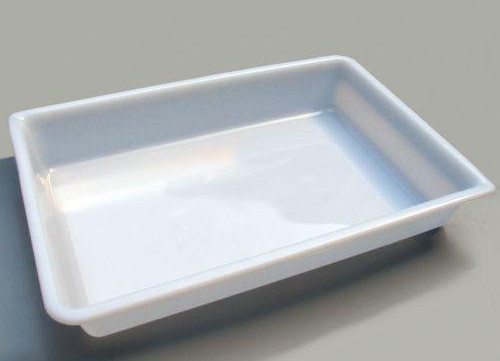
\includegraphics[width=\textwidth]{capitulo-5/graphics/bandeja-muestra.jpg}
            \caption{Bandeja de muestra vacía, sin larvas.}
    \end{subfigure}
    ~~~~
    \begin{subfigure}[b]{0.4\textwidth}
            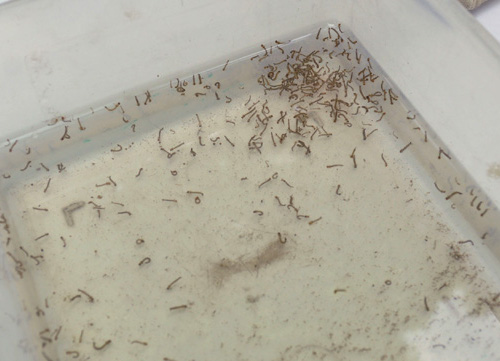
\includegraphics[width=\textwidth]{capitulo-5/graphics/larvas-dengue.jpg}
            \caption{Bandeja con larvas correspondientes al un punto de control.}

    \end{subfigure}
    \caption{\label{fig:cap5-conteo-pdi-bandejas} Bandejas de plástico utilizadas como contenedor
    de larvas.}
\end{figure}


Existen diferentes métodos para el análisis de imágenes que nos permiten realizar el conteo de
larvas teniendo en cuenta las características de las larvas. Presentaremos el método y las técnicas
utilizadas para la realizar el conteo de forma trivial, pero dista mucho de ser trivial y un
análisis más profundo escapa al alcance de este proyecto.

El método seleccionado para realizar el conteo fue el de Otsu, ya que no requiere supervisión
humana ni información previa de la imagen antes de su procesamiento \cite{santillan2008deteccion}.
Este método se emplea cuando hay una clara diferencia entre los objetos a extraer respecto del
fondo de la escena \citep{santillan2008deteccion}. Con la finalidad de resaltar las características
de las larvas, estas deben depositarse en una bandeja de plástico de color blanco para
posteriormente realizar la captura (\figref{fig:cap5-conteo-pdi-bandejas}), con esto se consigue
un contraste entre el fondo las larvas observadas.

\begin{figure}[!htbp]
    \centering
    \begin{subfigure}[b]{0.4\textwidth}
            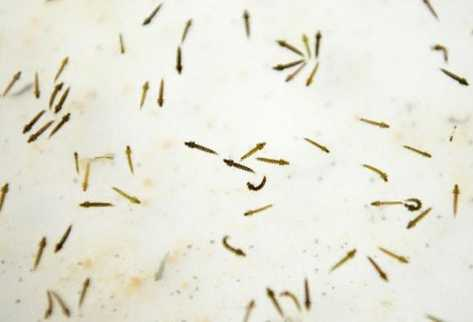
\includegraphics[width=\textwidth]{capitulo-5/graphics/larvas-original.png}
            \caption{Imagen original antes de la transformación.}
    \end{subfigure}
    ~~~~
    \begin{subfigure}[b]{0.4\textwidth}
            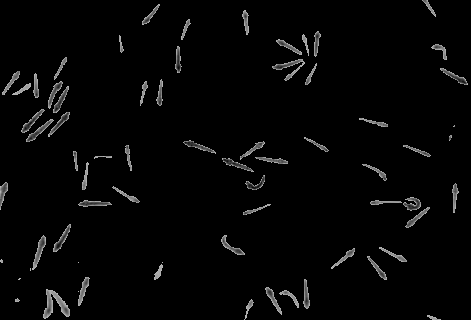
\includegraphics[width=\textwidth]{capitulo-5/graphics/larvas-otsu.png}
            \caption{Imagen luego de la umbralización de Otsu.}

    \end{subfigure}
    \caption{\label{fig:cap5-larvas-otsu} Transformación de una imagen mediante el método de
    Otsu.}
\end{figure}

La imagen se transforma a escala de grises, se ajusta el histograma para mejorar su contraste y se
calcula su umbral mediante el método de Otsu (\figref{fig:cap5-larvas-otsu}). Se definen 2
conjuntos, el primero corresponde a los objetos dentro de la imagen, en este caso las larvas, y el
segundo al el fondo, recipiente con el agua que contiene las larvas.  Se analiza simplemente el
nivel de gris correspondiente a cada píxel y se determina si forma parte de un objeto de estudio o
si forma parte del fondo.
